\documentclass{beamer}[10]

\usepackage{graphicx}
\usepackage{xcolor}
\usepackage{tabto}
%\usepackage{beamerthemesplit}
\usepackage{tikz}
\usepackage{cancel}
\usepackage{verbatim}
\usepackage{fancybox}
\usepackage{enumerate}
\usepackage{amsmath,amssymb,amsthm,textcomp,mathtools}
\usepackage[super]{nth}
\usepackage[amssymb]{SIunits}
\usepackage{booktabs}
\usepackage{cancel}
\usepackage{bm}
\usepackage[utf8]{inputenc}
\usepackage{tabularx}
\usepackage{ragged2e}
\newcolumntype{Y}{ >{\RaggedRight\arraybackslash}X}
\usetikzlibrary{arrows,shapes}
\newcommand\T{\rule{0pt}{2.6ex}}
\newcommand\B{\rule[-1.2ex]{0pt}{0pt}}
\definecolor{UUcrimson}{RGB}{204,0,0}
\mode<presentation>
{ \usetheme{default}
  \usecolortheme[named=UUcrimson]{structure}
  \useinnertheme{circles}
  \setbeamercovered{transparent}
  \setbeamertemplate{blocks}[rounded]
  \usefonttheme[onlymath]{serif}
  \setbeamertemplate{navigation symbols}{}
  \setbeamertemplate{footline}[page number]
  \setbeamertemplate{navigation symbols}{}
  \setbeamercolor{section in toc}{fg=black,bg=white}
  \setbeamercolor{alerted text}{fg=UUcrimson!80!gray}
  \setbeamercolor*{palette primary}{fg=white,bg=UUcrimson}
  \setbeamercolor*{palette secondary}{fg=UUcrimson!70!black,bg=gray!15!white}
  \setbeamercolor*{palette tertiary}{bg=UUcrimson!80!black,fg=gray!10!white}
  \setbeamercolor*{palette quaternary}{fg=UUcrimson,bg=gray!5!white}
  \setbeamercolor*{palette sidebar primary}{fg=UUcrimson!10!black}
  \setbeamercolor*{palette sidebar secondary}{fg=white}
  \setbeamercolor*{palette sidebar tertiary}{fg=UUcrimson!50!black}
  \setbeamercolor*{palette sidebar quaternary}{fg=gray!10!white}
  \setbeamercolor{titlelike}{parent=palette primary,fg=white}
  \setbeamercolor{frametitle}{bg=UUcrimson}
  \setbeamercolor{frametitle right}{bg=UUcrimson}
  \setbeamercolor*{separation line}{}
  \setbeamercolor*{fine separation line}{}
}

\usetikzlibrary{backgrounds}
\makeatletter
\tikzstyle{every picture}+=[remember picture]
\tikzset{%
  fancy quotes/.style={
    text width=\fq@width pt,
    align=justify,
    inner sep=1em,
    anchor=north west,
    minimum width=\linewidth,
    font=\itshape
  },
  fancy quotes width/.initial={.8\linewidth},
  fancy quotes marks/.style={
    scale=8,
    text=white,
    inner sep=0pt,
  },
  fancy quotes opening/.style={
    fancy quotes marks,
  },
  fancy quotes closing/.style={
    fancy quotes marks,
  },
  fancy quotes background/.style={
    show background rectangle,
    inner frame xsep=0pt,
    background rectangle/.style={
      fill=gray!25,
      rounded corners,
    },
  }
}
\newenvironment{fancyquotes}[1][]{%
\noindent
\tikzpicture[fancy quotes background]
\node[fancy quotes opening,anchor=north west] (fq@ul) at (0,0) {``};
\tikz@scan@one@point\pgfutil@firstofone(fq@ul.east)
\pgfmathsetmacro{\fq@width}{\linewidth - 2*\pgf@x}
\node[fancy quotes,#1] (fq@txt) at (fq@ul.north west) \bgroup}
{\egroup;
\node[overlay,fancy quotes closing,anchor=east] at (fq@txt.south east) {''};
\endtikzpicture}
\makeatother

\usepackage{scalerel}[2014/03/10]
\usepackage{stackengine}
\usepackage{empheq}
\newcommand*\widefbox[1]{\fbox{\hspace{0.5em}#1\hspace{0.5em}}}

\newcommand\reallywidetilde[1]{\ThisStyle{%
  \setbox0=\hbox{$\SavedStyle#1$}%
  \stackengine{-.1\LMpt}{$\SavedStyle#1$}{%
    \stretchto{\scaleto{\SavedStyle\mkern.2mu\sim}{.5467\wd0}}{.4\ht0}%
%    .2mu is the kern imbalance when clipping white space
%    .5467++++ is \ht/[kerned \wd] aspect ratio for \sim glyph
  }{O}{c}{F}{T}{S}%
}}
\usepackage{media9}

\logo{
\includegraphics[width=0.75cm]{logo.jpg}}
\author[Gibbs]{Dr. Jeremy A. Gibbs}
\institute{Department of Mechanical Engineering\\University of Utah}
\date{Fall 2016}
\title{LES of Turbulent Flows: Lecture 11}
\begin{document}

%----------------------------------------------------------------------------------------
%	TITLE & TOC SLIDES
%----------------------------------------------------------------------------------------

\begin{frame} 
  \titlepage
\end{frame}

%------------------------------------------------

\begin{frame}
\frametitle{Overview}
\tableofcontents
\end{frame}

%------------------------------------------------
\section{LES and numerical methods} %
%------------------------------------------------

\begin{frame}{LES and numerical methods}

\begin{itemize}
\item LES requires that the filtered equations of motion (see Lectures 6 and 7) be solved on a numerical grid
\item In LES we need to accurately represent high wavenumber turbulent fluctuations (small scale turbulence)
\item This means either we use high-order schemes (\textit{e.g.}, spectral methods) or we use fine grids with low-order schemes (\textit{e.g.}, \nth{2}-order central differences)
\end{itemize}

\end{frame}

%------------------------------------------------

\begin{frame}{LES and numerical methods}

\begin{itemize}
\item High-order schemes are more expensive, but for a given mesh they are more accurate (see Pope 571-579 for a discussion of resolving filtered fields)
\item Low-order finite difference (or volume) schemes provide flexibility of geometry but give rise to complications when modeling small scales motions
\item For more complete reviews of LES and numerics, see Guerts chapter 5 and Sagaut chapter 8.2, 8.3

\end{itemize}

\end{frame}

%------------------------------------------------

\begin{frame}{LES and numerical methods}

\begin{figure}
	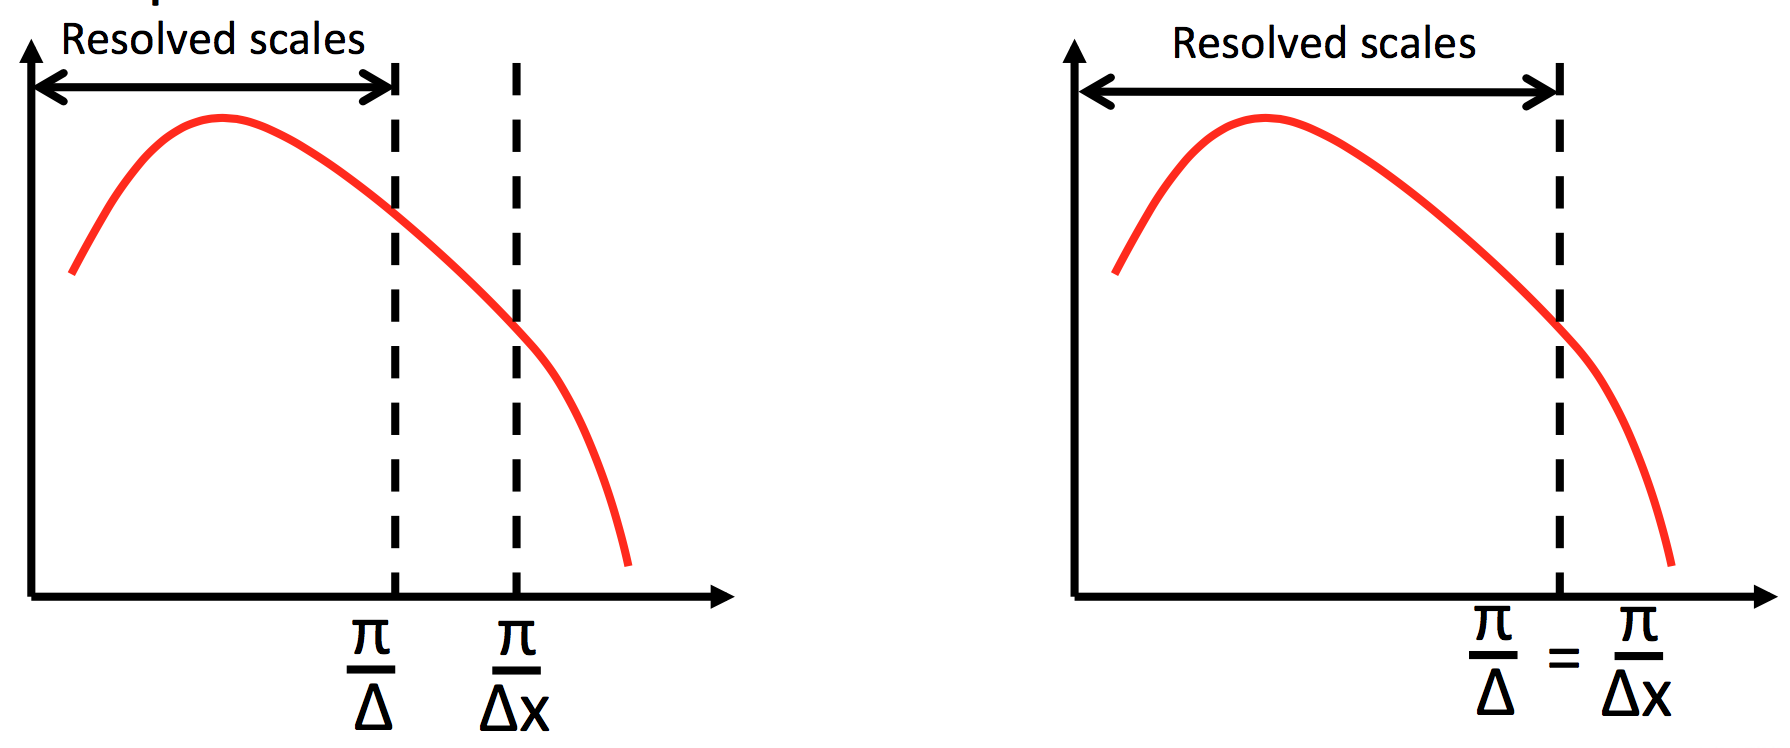
\includegraphics[width=\textwidth]{methods1}
\end{figure}

\end{frame}

%------------------------------------------------

\begin{frame}{LES and numerical methods}

\begin{itemize}
\item The filter applied in LES can be either \textbf{\textit{implicit}} or \textbf{\textit{explicit}}
\item \textbf{Implicit filtering:} The grid (or numerical basis) is assumed to be the LES low-pass
filter
\item \textbf{Explicit filtering:} A filter (typically box or Gaussian) is applied to the numerical grid (\textit{i.e.}, explicitly to the discretized N-S equations)
\end{itemize}

\end{frame}

%------------------------------------------------

\begin{frame}{LES and numerical methods}

\underline{Implicit filtering}
\begin{itemize}
\item \textbf{Pros:} takes full advantage of the numerical grid resolution
\item \textbf{Cons:} for some methods it is helpful to know the shape of the LES filter (this can be difficult to determine for some numerical methods). Truncation error can also become an issue.
\end{itemize}
\end{frame}

%------------------------------------------------

\begin{frame}{LES and numerical methods}

\underline{Explicit filtering}
\begin{itemize}
\item \textbf{Pros:} truncation error is reduced, filter shape is well defined
\item \textbf{Cons:} loss of resolution -- the total simulation time goes up as $\Delta_g^4$ (where $\Delta_g$ is the grid spacing) so maintaining the same space resolution as an implicit filter with  $\Delta_g/\Delta = 0.5$ will take $2^4=16$ more grid points
\end{itemize}
\end{frame}

%------------------------------------------------

\begin{frame}{LES and numerical methods}

\begin{itemize}
\item \textbf{Truncation errors can be on the order of SGS contributions} for low-order finite-difference schemes unless the filter width $\Delta$ is considerably larger than the grid spacing (see Ghosal 1996, Chow and Moin 2003)
\item Ghosal and Chow suggested a filter-to-grid ratio of 4 when using a \nth{2}-order centered scheme.
\end{itemize}
\end{frame}

%------------------------------------------------

\begin{frame}{LES and numerical methods}

Ghosal (1996) key findings
\begin{itemize}
\item Consider a von K\'{a}rm\'{a}n spectrum, \textit{e.g.},
$$E(k) = \frac{ak^4}{(b + k^2)^{17/6}}$$
The discretization error exceeds the subgrid error for \nth{2}-\nth{8}-order schemes. Additionally, for spectral schemes, the aliasing error (if 3/2 rule isn’t used) will dominate subgrid errors.

\item Reducing the ratio $C=\Delta_g/\Delta$ to values less than 1 reduces the error faster (by a factor of $C^{-3/4}$ than increasing the order of accuracy (a factor of 2 reduction when moving from \nth{2} to \nth{8})
\end{itemize}
\end{frame}

%------------------------------------------------

\begin{frame}{LES and numerical methods}

\begin{itemize}
\item \nth{2}-order schemes may have undesirable truncation errors (with respect to SFS model terms)
\item However, even-order schemes are non-dissipative
\item SFS models (on average) are purely dissipative
\item Therefore, \underline{all hope is not lost}!
\end{itemize}
\end{frame}

%------------------------------------------------

\begin{frame}{LES and numerical methods}

\begin{itemize}
\item The same is not true for odd-order schemes common in compressible flow solutions.
\item Examples include upwind-biased,  total variation diminishing (TVD), or fixed least squares (FLS) schemes
\item See \textit{Numerical Methods for Conservation Laws} by Leveque (1992) for a review of this numerical approach
\item Using these types of schemes with LES is somewhat controversial since their dissipative nature introduces an eddy viscosity like term to the solution (more later)

\end{itemize}
\end{frame}

%------------------------------------------------

\begin{frame}{LES and numerical methods}

\begin{itemize}
\item The total numerical dissipation in many cases introduced by upwind schemes is greater than that of SFS viscosity models (if no pre-filtering is performed) -- even for \nth{7}-order schemes (Beaudan and Moin, 1994)
\item For the Smagorinsky model (more later) Garnier et al. (1999) found that up to \nth{5}-order upwind schemes in decaying isotropic turbulence are more dissipative
\item For the Deardorff scheme, Gibbs and Fedorovich (2014b) found that the same result when applied to an atmospheric convective boundary layer (CBL)
\end{itemize}
\end{frame}

%------------------------------------------------

\begin{frame}{LES and numerical methods}

Gibbs and Fedorovich (2014b) overview
\begin{itemize}
\item Studied two idealized convective boundary layers -- one with a mean shear of $10\ \metre\ \reciprocal\second$ and the other with no mean shear
\item Each case was run with our traditional LES code (OU-LES) and the WRF model used in LES mode (WRF-LES) on identical $10.24\times 10.24 \times 2\ \kilo\metre^2$ numerical grids with $20$-$\metre$ spacing
\item OU-LES used \nth{2}-order centered finite difference approximations, WRF-LES used \nth{5}-order upwind-biased finite differences
\item Compared turbulence spectra and other statistics
\end{itemize}
\end{frame}

%------------------------------------------------

\begin{frame}{LES and numerical methods}

\begin{figure}
	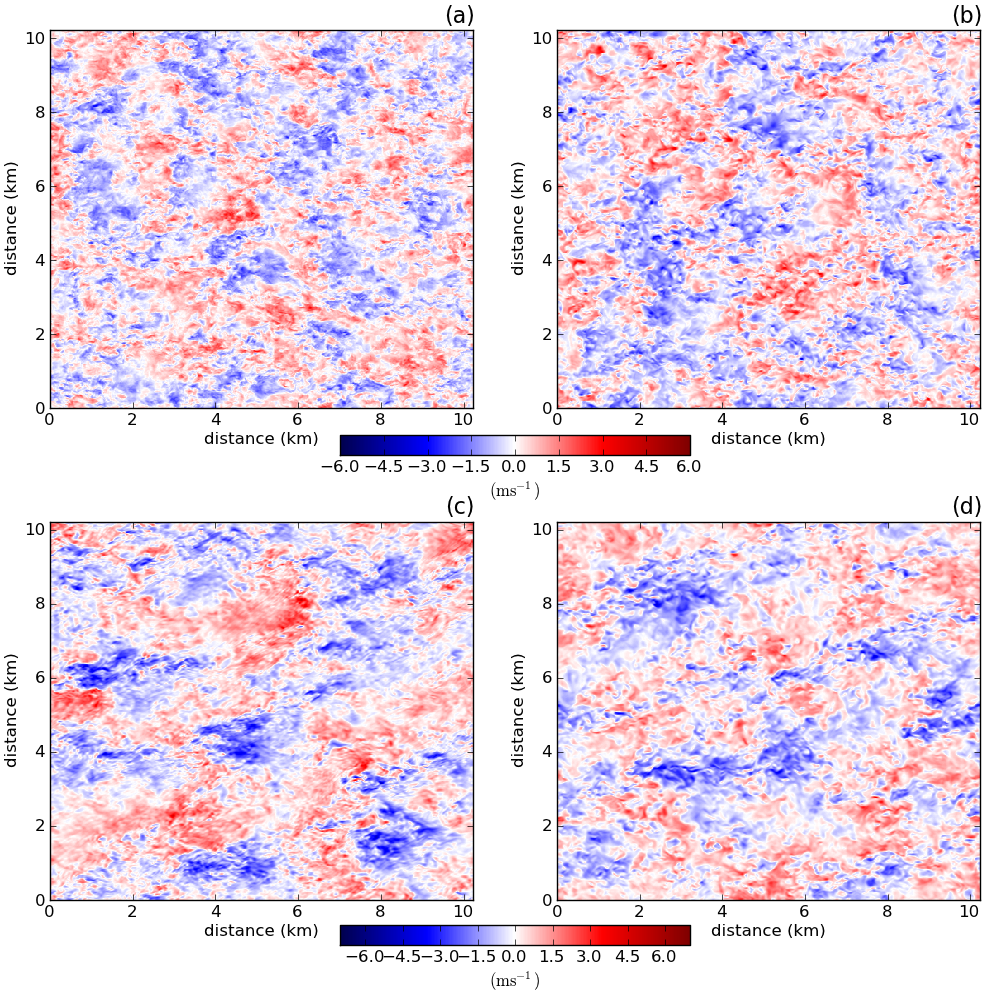
\includegraphics[width=0.67\textwidth]{gibbs1}
	\caption{\scriptsize \textit{u}-component velocity for shear-free (top) and shear-driven (bottom) from OU-LES (left) and WRF-LES (right) at $z/z_i=0.25$}
\end{figure}

\end{frame}

%------------------------------------------------

\begin{frame}{LES and numerical methods}

\begin{figure}
	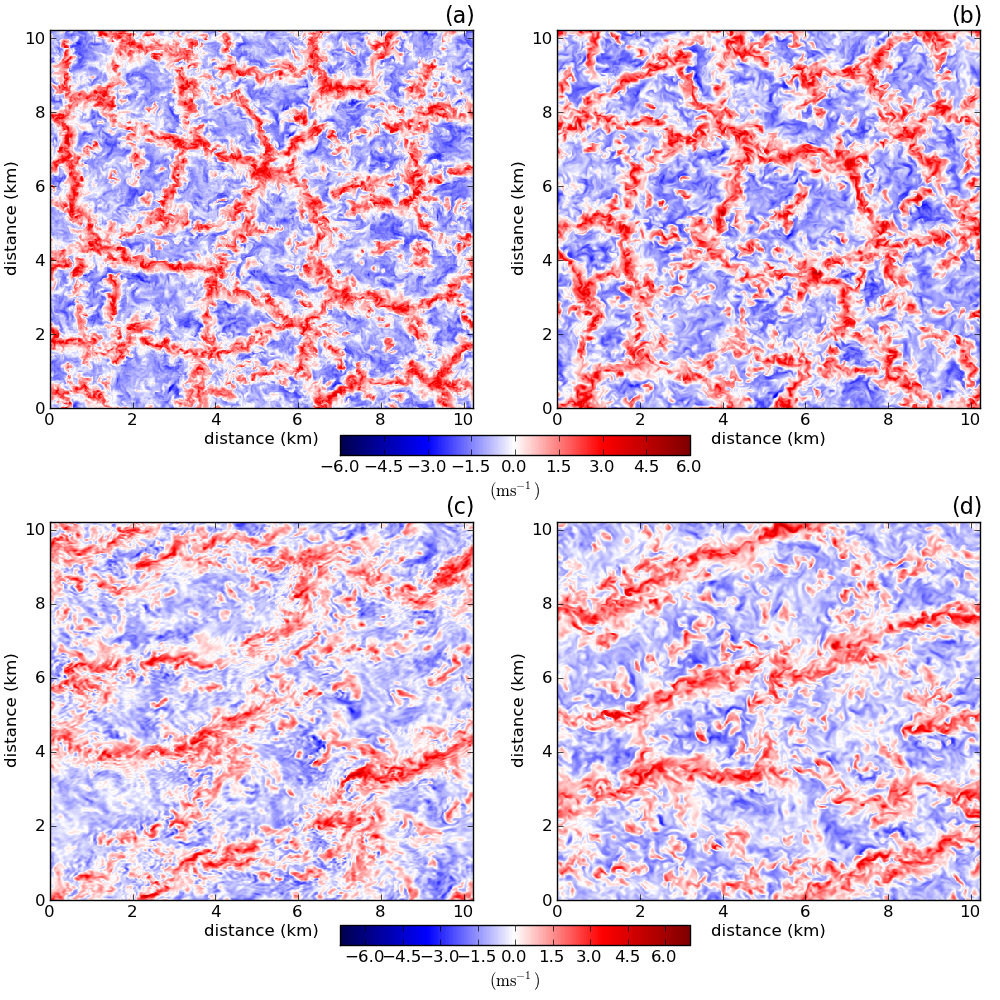
\includegraphics[width=0.67\textwidth]{gibbs2}
	\caption{\scriptsize \textit{w}-component velocity for shear-free (top) and shear-driven (bottom) from OU-LES (left) and WRF-LES (right) at $z/z_i=0.25$}
\end{figure}

\end{frame}

%------------------------------------------------

\begin{frame}{LES and numerical methods}

\begin{figure}
	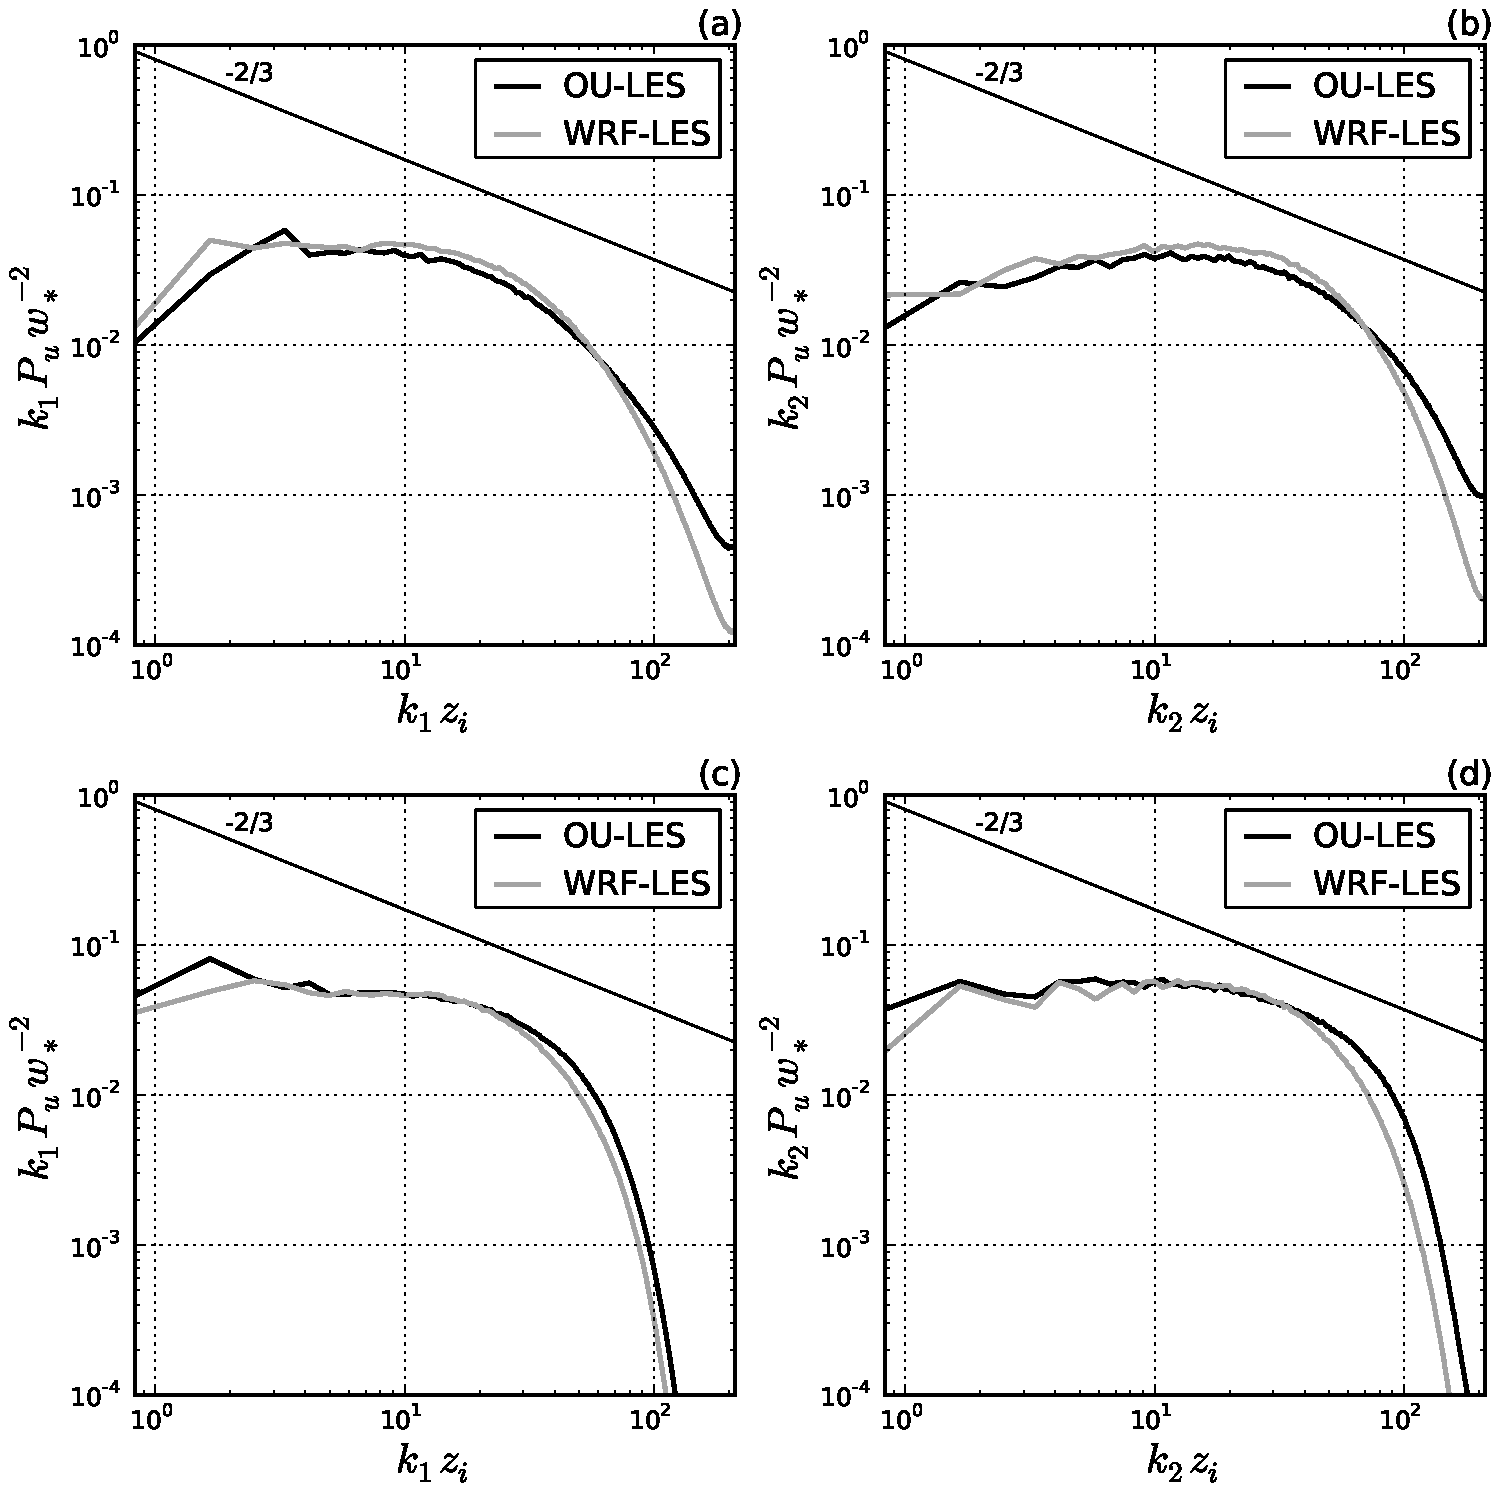
\includegraphics[width=0.67\textwidth]{gibbs3}
	\caption{\scriptsize normalized 1D \textit{u}-component spectra (left: \textit{x}-dir, right: \textit{y}-dir) for shear-free (top) and shear-driven (bottom) from OU-LES (left) and WRF-LES (right) at $z/z_i=0.25$}
\end{figure}

\end{frame}

%------------------------------------------------

\begin{frame}{LES and numerical methods}

\begin{figure}
	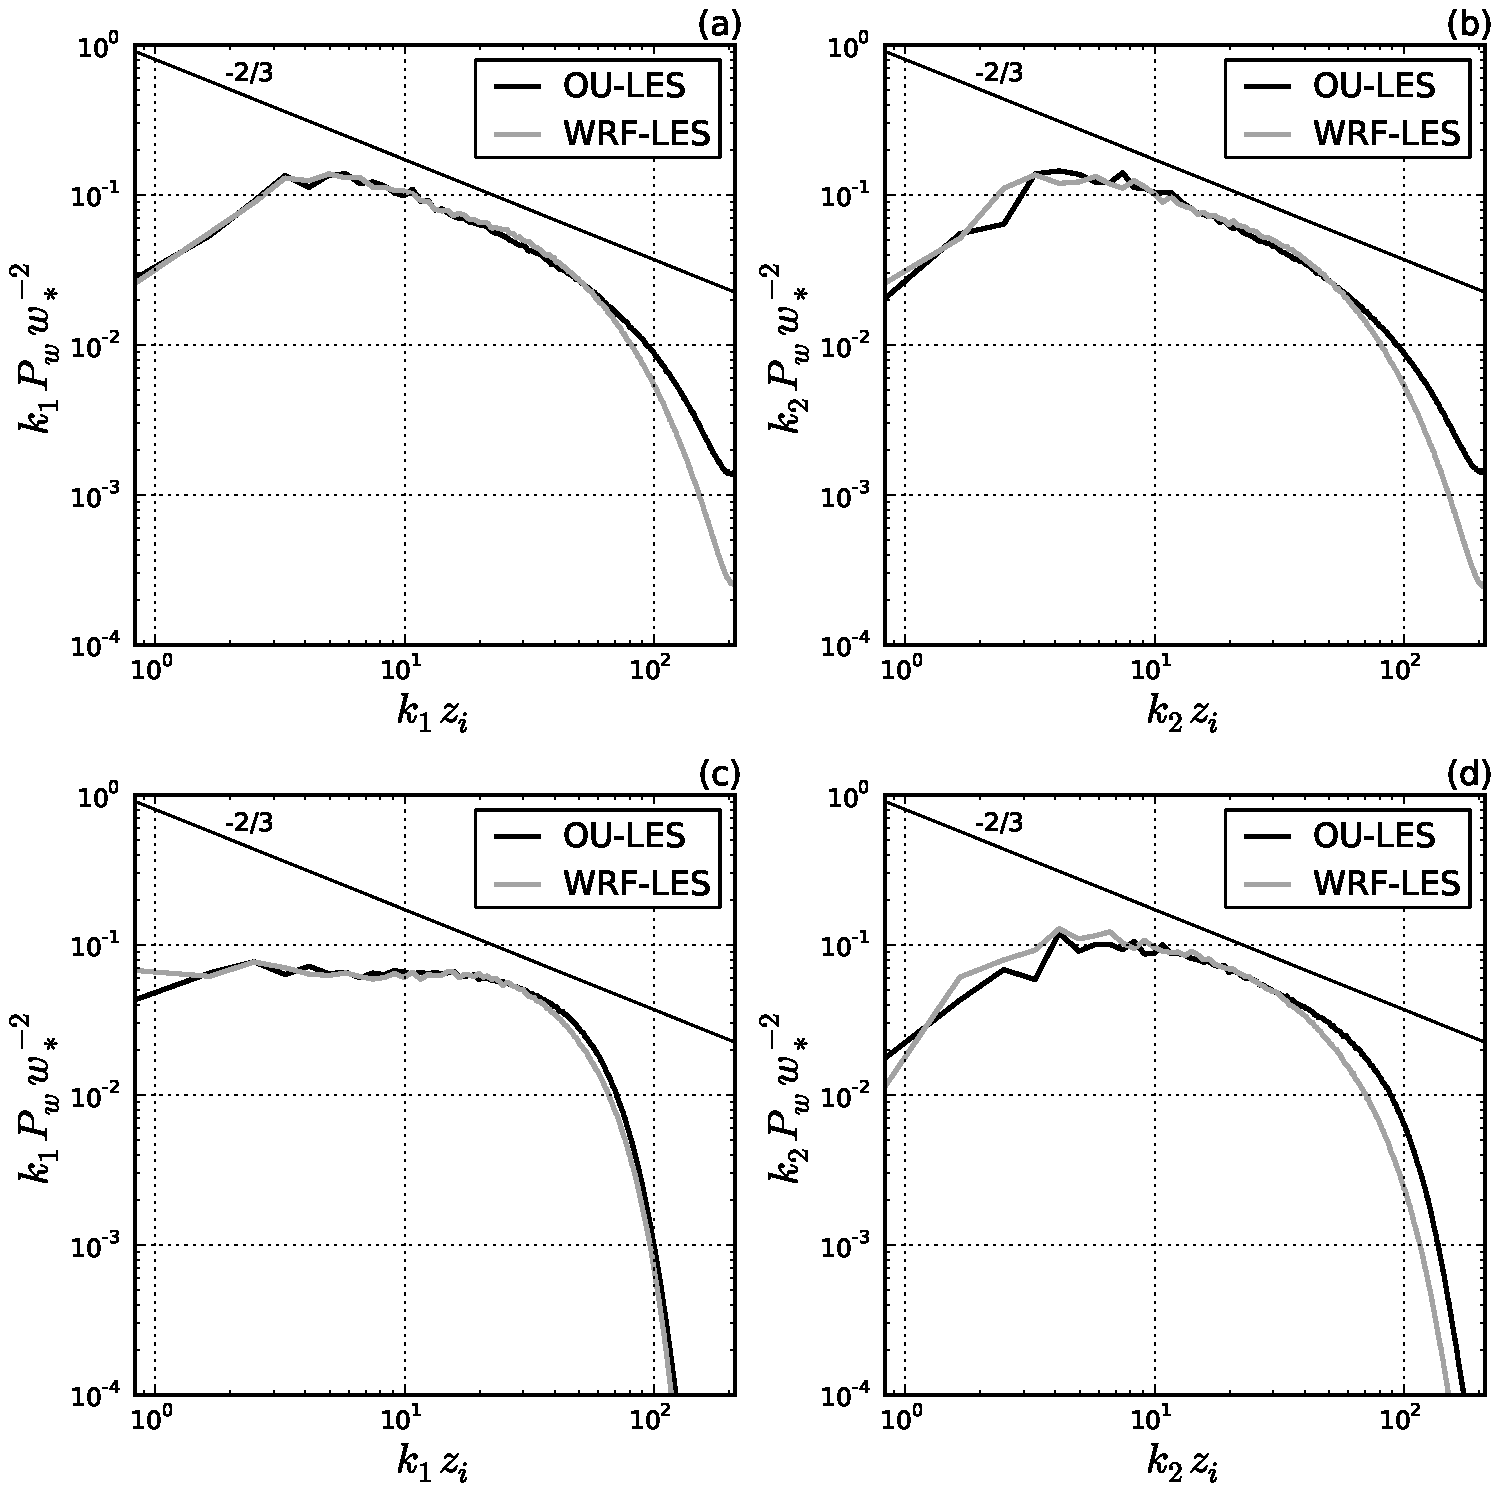
\includegraphics[width=0.67\textwidth]{gibbs4}
	\caption{\scriptsize normalized 1D \textit{w}-component spectra (left: \textit{x}-dir, right: \textit{y}-dir) for shear-free (top) and shear-driven (bottom) from OU-LES and WRF-LES at $z/z_i=0.25$}
\end{figure}

\end{frame}

%------------------------------------------------

\begin{frame}{LES and numerical methods}

\begin{figure}
	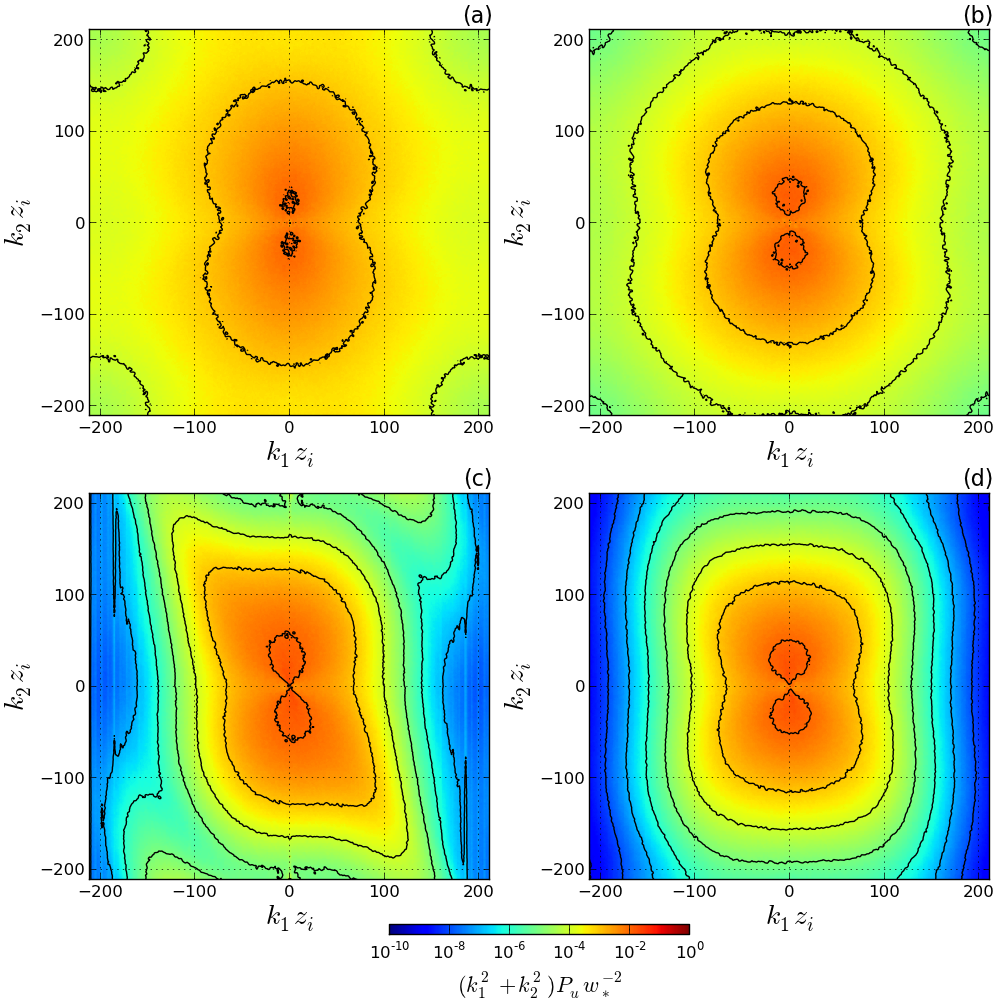
\includegraphics[width=0.67\textwidth]{gibbs5}
	\caption{\scriptsize normalized 2D \textit{u}-component spectra for shear-free (top) and shear-driven (bottom) from OU-LES (left) and WRF-LES (right) at $z/z_i=0.25$}
\end{figure}

\end{frame}

%------------------------------------------------

\begin{frame}{LES and numerical methods}

\begin{figure}
	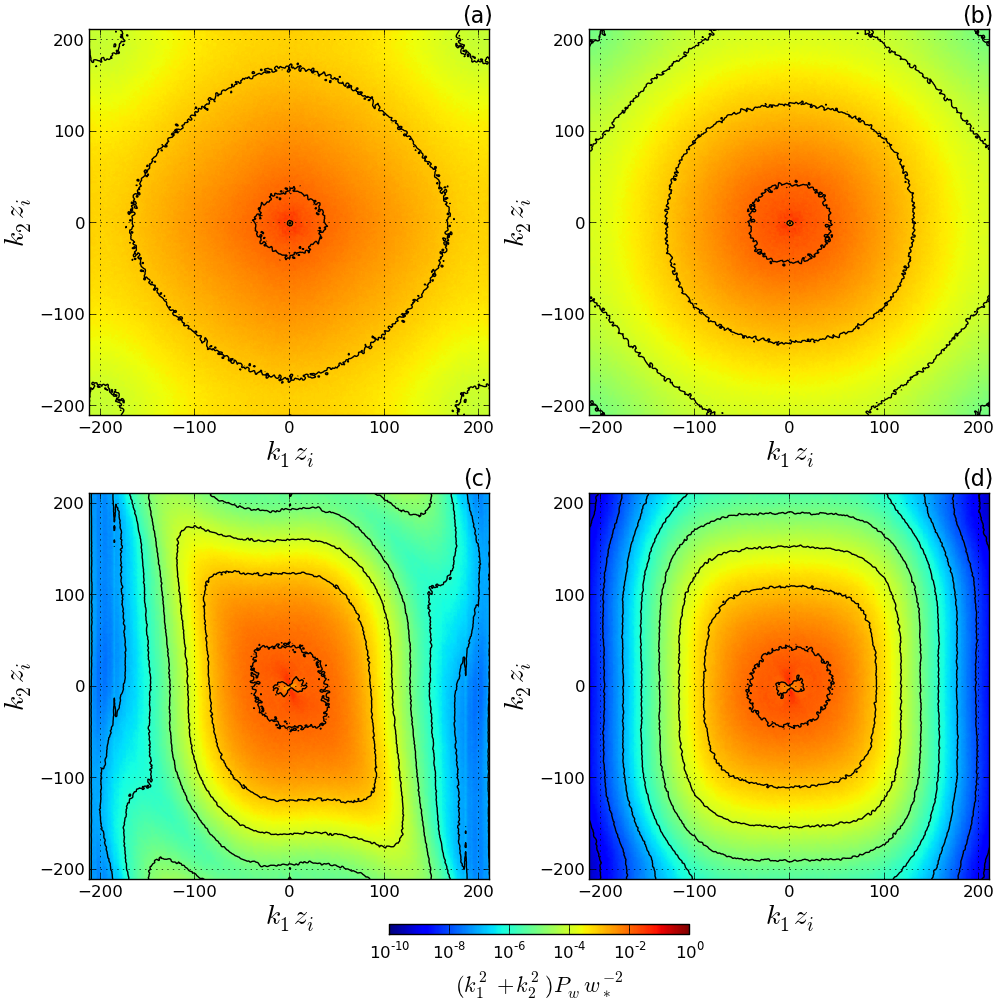
\includegraphics[width=0.67\textwidth]{gibbs6}
	\caption{\scriptsize normalized 2D \textit{w}-component spectra for shear-free (top) and shear-driven (bottom) from OU-LES (left) and WRF-LES (right) at $z/z_i=0.25$}
\end{figure}

\end{frame}


%------------------------------------------------

\begin{frame}{LES and numerical methods}

\begin{figure}
	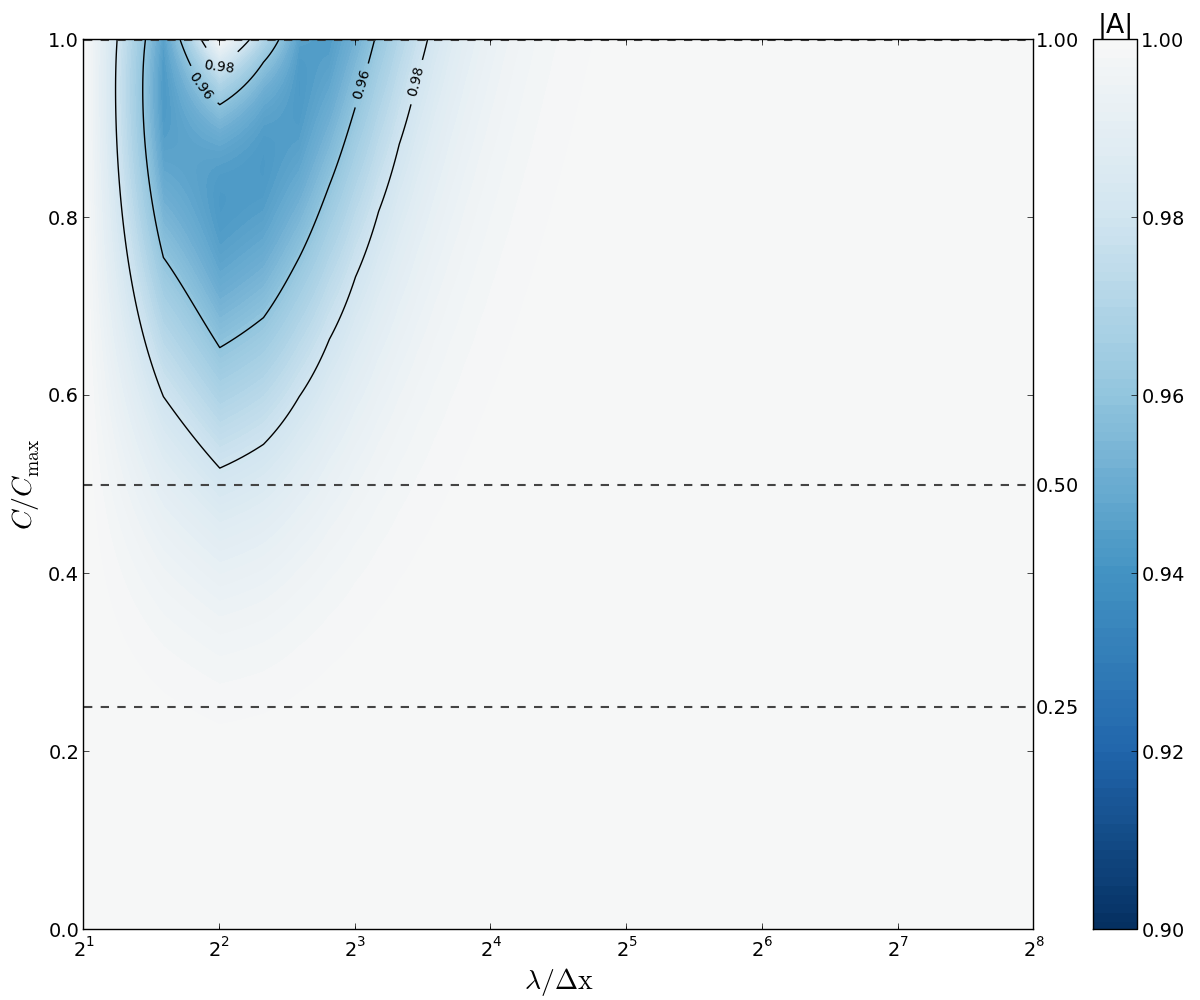
\includegraphics[width=0.8\textwidth]{gibbs7}
	\caption{\scriptsize Amplification factor for \nth{2}-order centered scheme with RK3 time scheme.}
\end{figure}

\end{frame}

%------------------------------------------------

\begin{frame}{LES and numerical methods}

\begin{figure}
	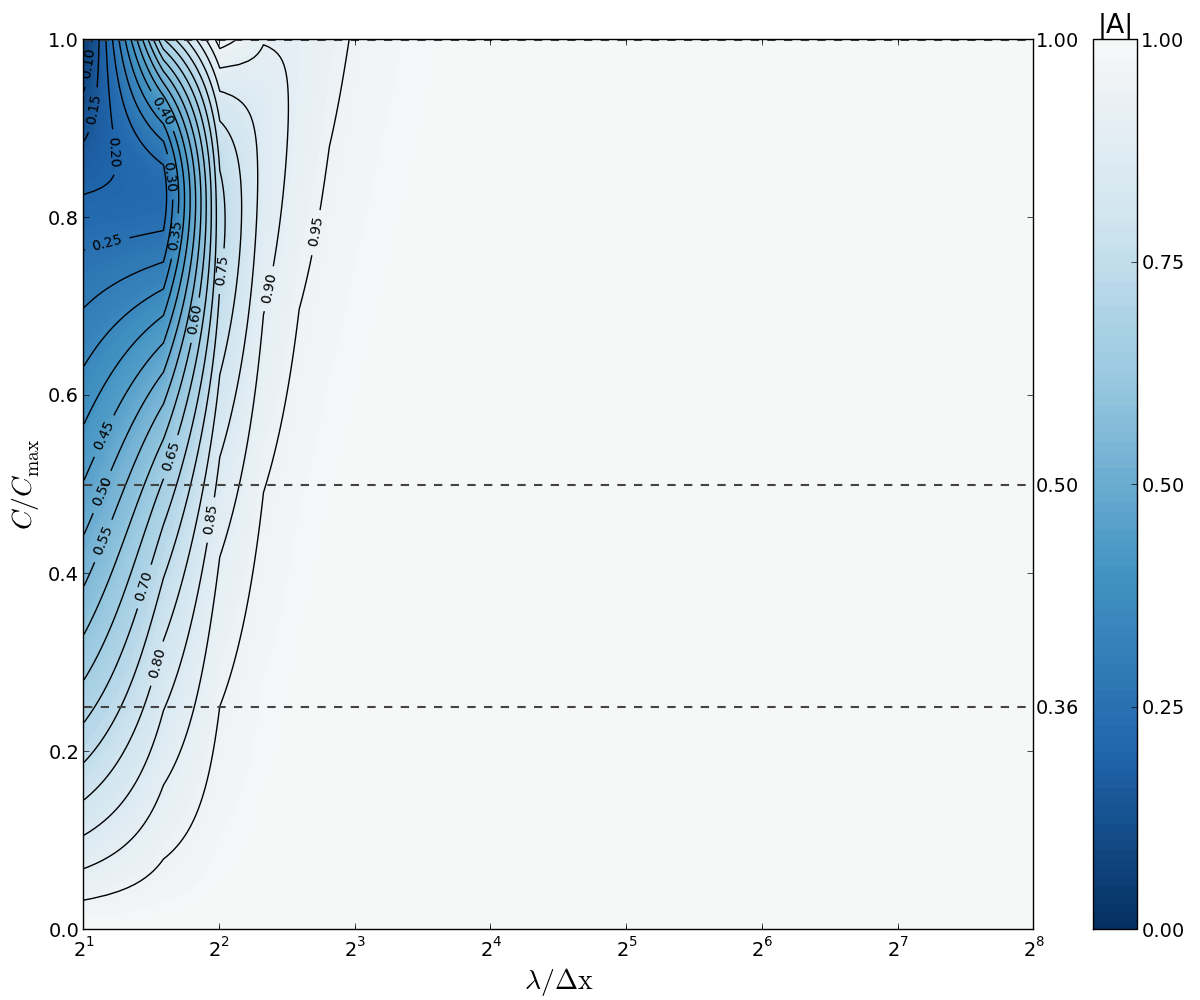
\includegraphics[width=0.8\textwidth]{gibbs8}
	\caption{\scriptsize Amplification factor for \nth{5}-order upwind scheme with RK3 time scheme.}
\end{figure}

\end{frame}


\begin{frame}{LES and numerical methods}

\begin{itemize}
\item Gibbs and Fedorovich (2014a) looked at the effect of time integration schemes on turbulence spectra and moments
\item You can see how many things complicate the understanding of LES results -- the model itself, the choice of cutoff scale, the model numerics, etc.
\item These items can also act to determine the spectral resolution of the simulation -- meaning what minimum scale of features is trustworthy from a theoretical and statistical standpoint
\end{itemize}
\end{frame}


%------------------------------------------------
\section{Subgrid-Scale Modeling} %
%------------------------------------------------

\begin{frame}{Subgrid-Scale Modeling}

\begin{itemize}
\item One of the major hurdles to making LES a reliable tool for engineering and environmental applications is the formulation of SGS models and the specification of model coefficients
\end{itemize}

\end{frame}

%------------------------------------------------

\begin{frame}{Subgrid-Scale Modeling}

\begin{columns}[T]
    \begin{column}{.6\textwidth}
      \begin{minipage}[c][.6\textheight][c]{\linewidth}
      \begin{itemize}
      \item Recall: we can define 3 different ``scale regions'' in LES\newline -- resolved scales \newline -- resolved SFS \newline -- SGSs
      \item We can also decompose a general variable as
      $$\phi=\widetilde{\phi} + \phi^{\prime}$$
      \end{itemize}
      \end{minipage}
    \end{column}
    \begin{column}{.6\textwidth}
    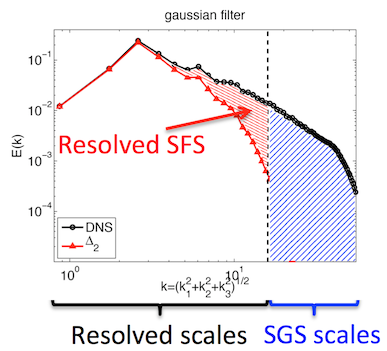
\includegraphics[width=0.95\textwidth]{decomp1}
    \end{column}
  \end{columns}

\end{frame}

%------------------------------------------------

\begin{frame}{Subgrid-Scale Modeling}

\begin{columns}[T]
    \begin{column}{.6\textwidth}
      \begin{minipage}[c][.6\textheight][c]{\linewidth}
      \begin{itemize}
      \item When we talk about SGS models we are specifically talking about the scales below $\Delta$ and \textbf{NOT}the resolved SFS
      \item We will specifically discuss the resolved SFSs when we talk about filter reconstruction later on (time permitting)
      \end{itemize}
      \end{minipage}
    \end{column}
    \begin{column}{.6\textwidth}
    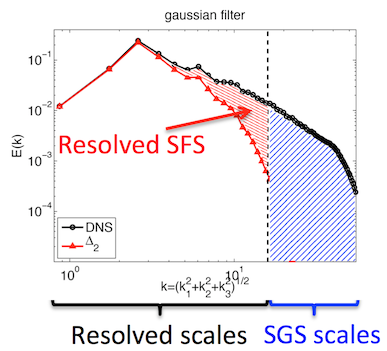
\includegraphics[width=0.95\textwidth]{decomp1}
    \end{column}
  \end{columns}

\end{frame}

%------------------------------------------------

\begin{frame}{Subgrid-Scale Modeling}

\begin{columns}[T]
    \begin{column}{.6\textwidth}
      \begin{minipage}[c][.6\textheight][c]{\linewidth}
      \begin{itemize}
      \item We will focus on LES with explicit SGS models
      \item A class of LES referred to as Implicit LES (ILES) also exists
      \item Note: these terms are different than implicit/explicit filtering
      \end{itemize}
      \end{minipage}
    \end{column}
    \begin{column}{.6\textwidth}
    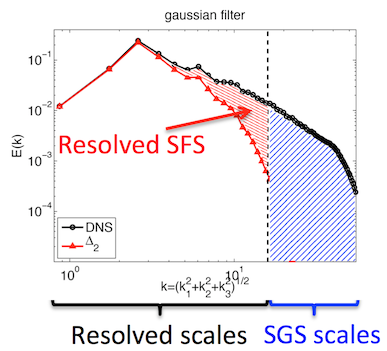
\includegraphics[width=0.95\textwidth]{decomp1}
    \end{column}
  \end{columns}
\end{frame}

%------------------------------------------------

\begin{frame}{Subgrid-Scale Modeling}

\begin{columns}[T]
    \begin{column}{.6\textwidth}
      \begin{minipage}[c][.6\textheight][c]{\linewidth}
      \begin{itemize}
      \item ILES was first developed for compressible flow
      \item ILES methods are numerical methods that capture the energy-containing and inertial ranges of turbulent flows, while relying on their own intrinsic dissipation to act as a subgrid model
      \end{itemize}
      \end{minipage}
    \end{column}
    \begin{column}{.6\textwidth}
    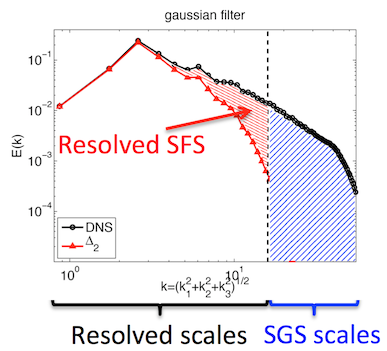
\includegraphics[width=0.95\textwidth]{decomp1}
    \end{column}
  \end{columns}
\end{frame}

%------------------------------------------------

\begin{frame}{Subgrid-Scale Modeling}

\begin{columns}[T]
    \begin{column}{.6\textwidth}
      \begin{minipage}[c][.6\textheight][c]{\linewidth}
      \begin{itemize}
      \item ILES assumes the SGSs are purely dissipative and act in a similar way to dissipative numerical schemes
      \item In general, ILES uses monotinicity-preserving numerical schemes
      \item See Grinstein \textit{et al.} (2007) on Canvas and website
      \end{itemize}
      \end{minipage}
    \end{column}
    \begin{column}{.6\textwidth}
    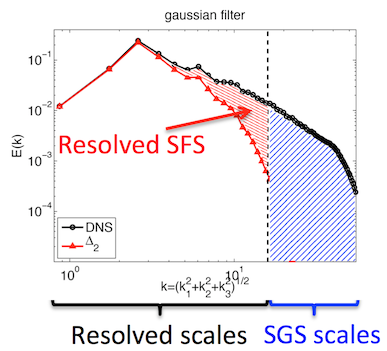
\includegraphics[width=0.95\textwidth]{decomp1}
    \end{column}
  \end{columns}
\end{frame}

%------------------------------------------------
\section{Modeling $\tau_{ij}$}
%------------------------------------------------
\begin{frame}{Modeling $\tau_{ij}$}

\begin{itemize}
\item Our discussion of modeling $\tau_{ij}$ will follow Sagaut (pages 49-50, 59-60) and Pope (pages 582-583)
\item We can decompose the nonlinear term as follows by using $\phi=\widetilde{\phi} + \phi^{\prime}$
\begin{align*}
\widetilde{u_i u_j} &= \reallywidetilde{\left(\widetilde{u_i} + u_i^{\prime}\right)\left(\widetilde{u_j} + u_j^{\prime}\right)}\\
&=\widetilde{\widetilde{u_i}\widetilde{u_j}} + \widetilde{\widetilde{u_i}u_j^{\prime}} + \widetilde{\widetilde{u_j}u_i^{\prime}} + \widetilde{u_i^{\prime}u_j^{\prime}}
\end{align*}
\end{itemize}
\end{frame}

%------------------------------------------------
\begin{frame}{Modeling $\tau_{ij}$}
\begin{align*}
\widetilde{u_i u_j} &= \reallywidetilde{\left(\widetilde{u_i} + u_i^{\prime}\right)\left(\widetilde{u_j} + u_j^{\prime}\right)}\\
&=\widetilde{\widetilde{u_i}\widetilde{u_j}} + \widetilde{\widetilde{u_i}u_j^{\prime}} + \widetilde{\widetilde{u_j}u_i^{\prime}} + \widetilde{u_i^{\prime}u_j^{\prime}}
\end{align*}
\begin{itemize}
\item We now have the nonlinear term as a function of $\widetilde{u_i}$ and $\widetilde{u_i^{\prime}}$
\item Two different basic forms of the decomposition (based on the above equation) are prevalent
\end{itemize}
\end{frame}

%------------------------------------------------
\begin{frame}{Modeling $\tau_{ij}$}

\begin{itemize}
\item The first one is based on the idea that all terms appearing in the evolution of a filtered quantity should be filtered
$$\tau_{ij} = \boxed{C_{ij} + R_{ij}} = \widetilde{u_iu_j} - \widetilde{\widetilde{u_i}\widetilde{u_j}}$$
\begin{align*}
	\mbox{where}\quad C_{ij} &= \widetilde{\widetilde{u_i} u_j^{\prime}} + \widetilde{\widetilde{u_j} u_i^{\prime}} &\Rightarrow & \parbox{14em}{interaction between resolved and SFSs}\\
	\mbox{and} \quad R_{ij} &= \widetilde{u_i^{\prime}u_j^{\prime}} &\Rightarrow & \parbox{14em}{SFS ``Reynold's'' stress}
\end{align*}
\end{itemize}
\end{frame}

%------------------------------------------------
\begin{frame}{Modeling $\tau_{ij}$}

\begin{itemize}
\item A second definition can be obtained by further decomposition of $\widetilde{\widetilde{u_i}\widetilde{u_j}}$
$$\widetilde{\widetilde{u_i}\widetilde{u_j}} = \underbrace{\left( \widetilde{\widetilde{u_i}\widetilde{u_j}} - \widetilde{u_i} \widetilde{u_j}\right)}_{L_{ij}} + \widetilde{u_i} \widetilde{u_j}$$
$$\mbox{where}\quad L_{ij} \Rightarrow \parbox{20em}{Leonard stress -- the interaction among the smallest resolved scales)}$$
Our total decomposition is now $$\boxed{\tau_{ij} = L_{ij} + C_{ij} + R_{ij}} = \widetilde{u_iu_j} - \widetilde{u_i}\widetilde{u_j}$$
\item See Leonard (1974)
\end{itemize}
\end{frame}

%------------------------------------------------
\begin{frame}{Modeling $\tau_{ij}$}
$$\tau_{ij} = L_{ij} + C_{ij} + R_{ij}$$
\begin{itemize}
\item If our filter is a Reynold's operator, the $C_{ij}$ and $L_{ij}$ vanish
\item \textbf{Note:} while $\tau_{ij}$ and $R_{ij}$ are invariant to Galilean transformations, $L_{ij}$ and $C_{ij}$ are not (see Speziale 1985)
\item As a result, the decomposition given above (for the most part) is not used anymore
\item However, we will see similar terms again in our SGS models
\end{itemize}
\end{frame}

%------------------------------------------------
\begin{frame}{Modeling $\tau_{ij}$}
\begin{itemize}
\item Germano purposed a more rigorous decomposition into generalized filtered moments
\item Under this framework, the generalized moments look just like ``Reynolds'' moments, our original $\tau_{ij}$
\item See Germano (1992) on Canvas and website
\item This is also recommended reading for a discussion of filtering and the relationship between LES filters and Reynolds operators
\end{itemize}
\end{frame}

%------------------------------------------------

\end{document}

